\section*{Ход выполнения}

\paragraph{}
В таблице 1 приведены выбранные матрицы из ресурса: \href{https://sparse.tamu.edu/}{sparse.tamu.edu}\\

\begin{table}[t]
    \renewcommand{\tablename}{Таблица}
    \caption{выбранные матрицы}
    \begin{tabularx}{0.8\textwidth}{
        | >{\centering\arraybackslash}X
        | >{\centering\arraybackslash}X
        | >{\centering\arraybackslash}X |
    }
        \hline
        Название       & Размер           & Количество ненулевых элементов \\
        \hline
        Dubcova2       & 62025 на 65025   & 1030225                        \\
        \hline
        finan512       & 74752 на 74752   & 596992                         \\
        \hline
        G2\_circuit    & 150102 на 150102 & 726674                         \\
        \hline
        qa8fm          & 66127 на 66127   & 1660579                        \\
        \hline
        thermomech\_dM & 204316 на 204316 & 1423116                        \\
        \hline
    \end{tabularx}\label{tab:table2}
\end{table}\\

Все вычисления проводились с точностью 10-8 и количеством итераций до 20000. Все скрипты для каждого метода представлены в приложении А.

На рисунках 1-11 приведены истории невязок для матрицы Dubcova2


\begin{figure}[H]
    \renewcommand{\figurename}{Рисунок}
    \centering{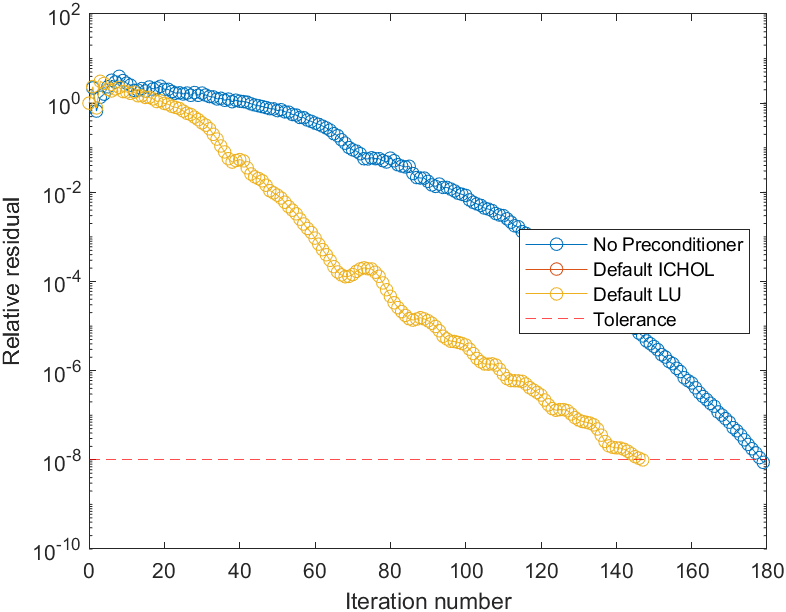
\includegraphics[scale=0.70]{img/dupcova/bicg}}
    \caption{История невязок методом bicg для матрицы Dubcova2}
    \label{fig:image_1}
\end{figure}

\begin{figure}[H]
    \renewcommand{\figurename}{Рисунок}
    \centering{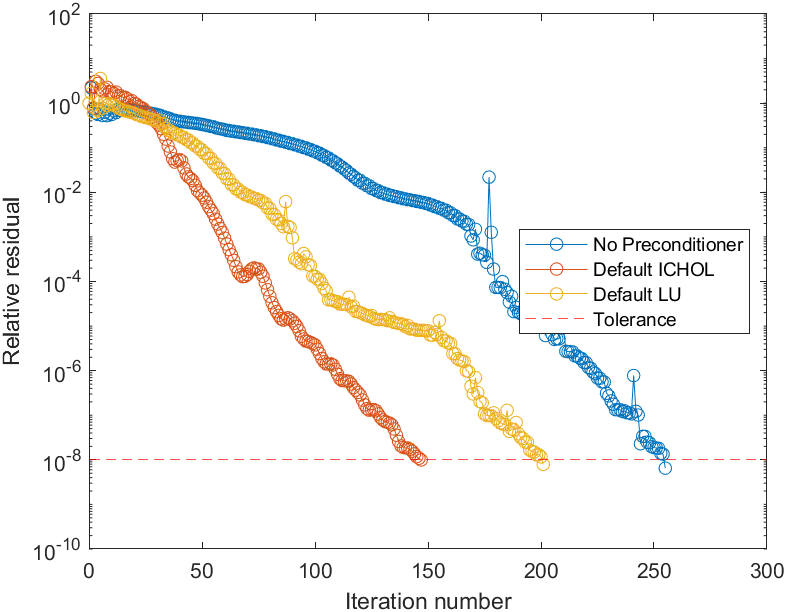
\includegraphics[scale=0.70]{img/dupcova/bicgstab}}
    \caption{История невязок методом bicgstab для матрицы Dubcova2}
    \label{fig:image_2}
\end{figure}

\begin{figure}[H]
    \renewcommand{\figurename}{Рисунок}
    \centering{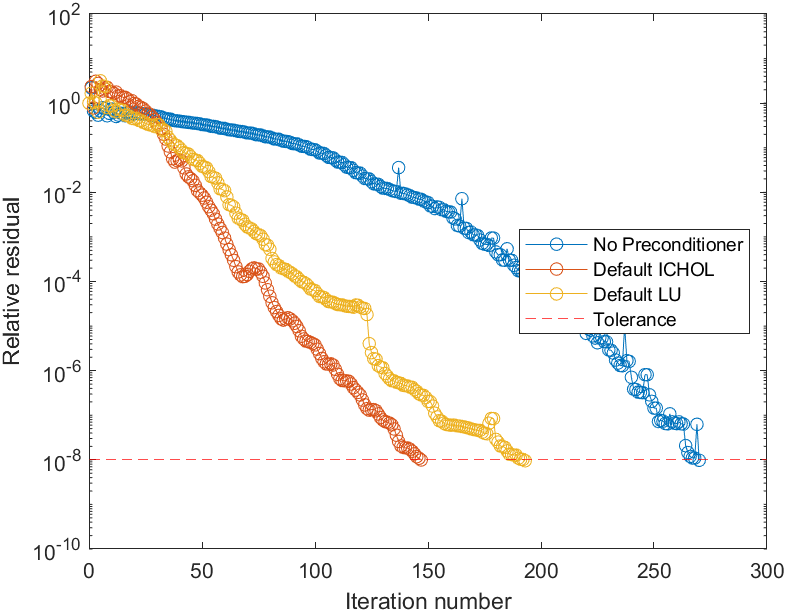
\includegraphics[scale=0.70]{img/dupcova/bicgstabl}}
    \caption{История невязок методом bicgstabl для матрицы Dubcova2}
    \label{fig:image_3}
\end{figure}

\begin{figure}[H]
    \renewcommand{\figurename}{Рисунок}
    \centering{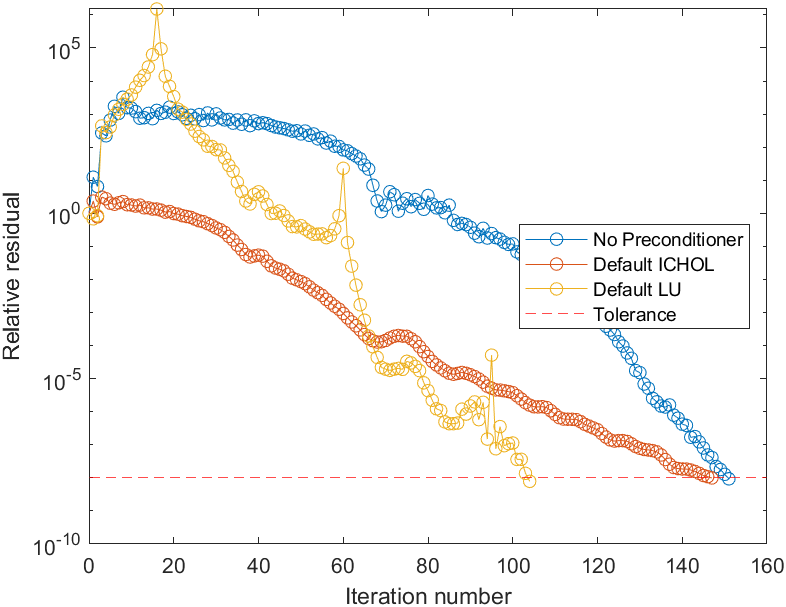
\includegraphics[scale=0.70]{img/dupcova/cgs}}
    \caption{История невязок методом cgs для матрицы Dubcova2}
    \label{fig:image_4}
\end{figure}

\begin{figure}[H]
    \renewcommand{\figurename}{Рисунок}
    \centering{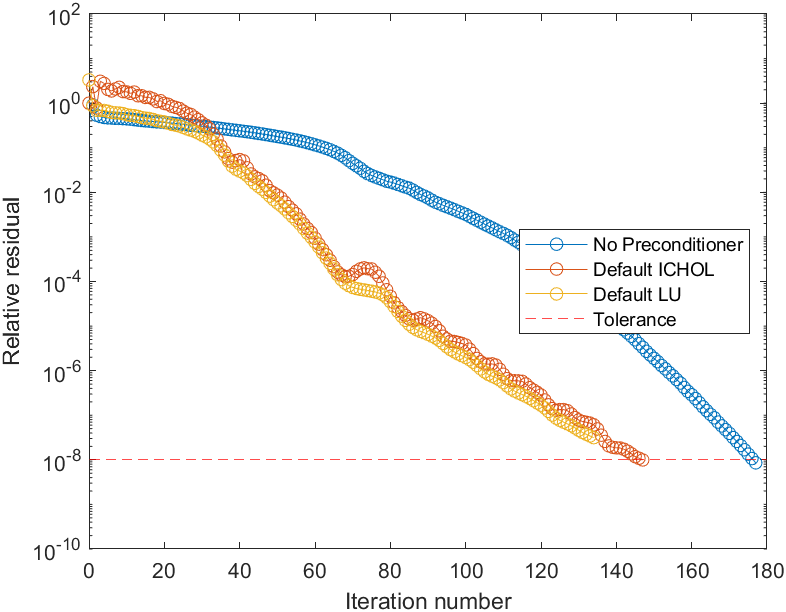
\includegraphics[scale=0.70]{img/dupcova/gmres}}
    \caption{История невязок методом gmres для матрицы Dubcova2}
    \label{fig:image_5}
\end{figure}

\begin{figure}[H]
    \renewcommand{\figurename}{Рисунок}
    \centering{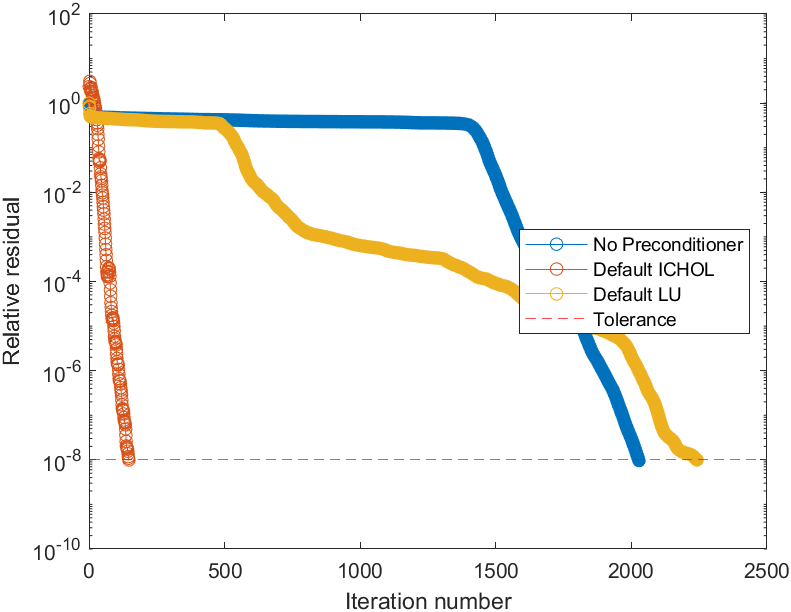
\includegraphics[scale=0.70]{img/dupcova/lsqr}}
    \caption{История невязок методом lsqr для матрицы Dubcova2}
    \label{fig:image_6}
\end{figure}

\begin{figure}[H]
    \renewcommand{\figurename}{Рисунок}
    \centering{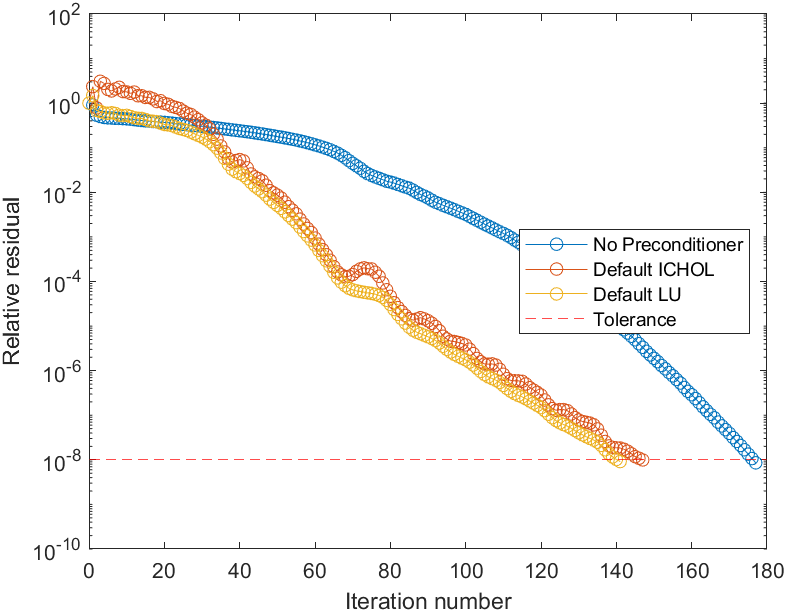
\includegraphics[scale=0.70]{img/dupcova/minres}}
    \caption{История невязок методом minres для матрицы Dubcova2}
    \label{fig:image_7}
\end{figure}

\begin{figure}[H]
    \renewcommand{\figurename}{Рисунок}
    \centering{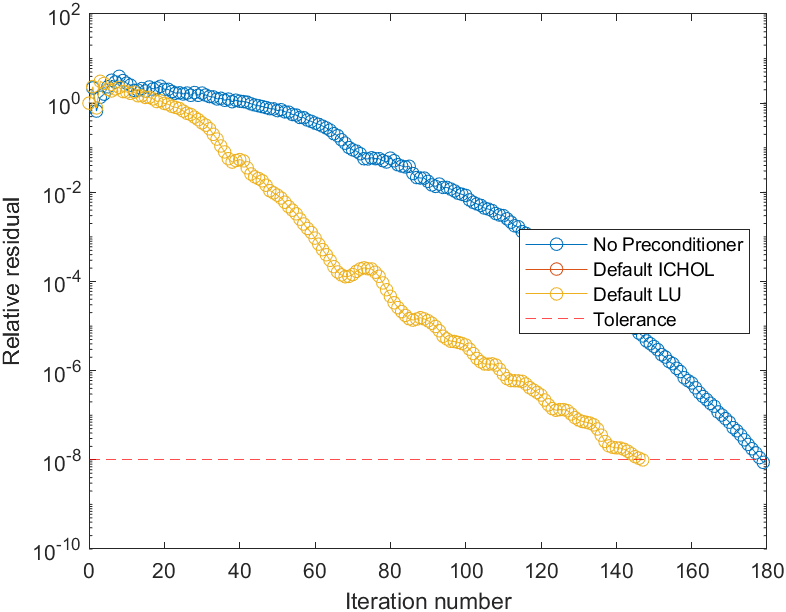
\includegraphics[scale=0.70]{img/dupcova/pcg}}
    \caption{История невязок методом pcg для матрицы Dubcova2}
    \label{fig:image_8}
\end{figure}

\begin{figure}[H]
    \renewcommand{\figurename}{Рисунок}
    \centering{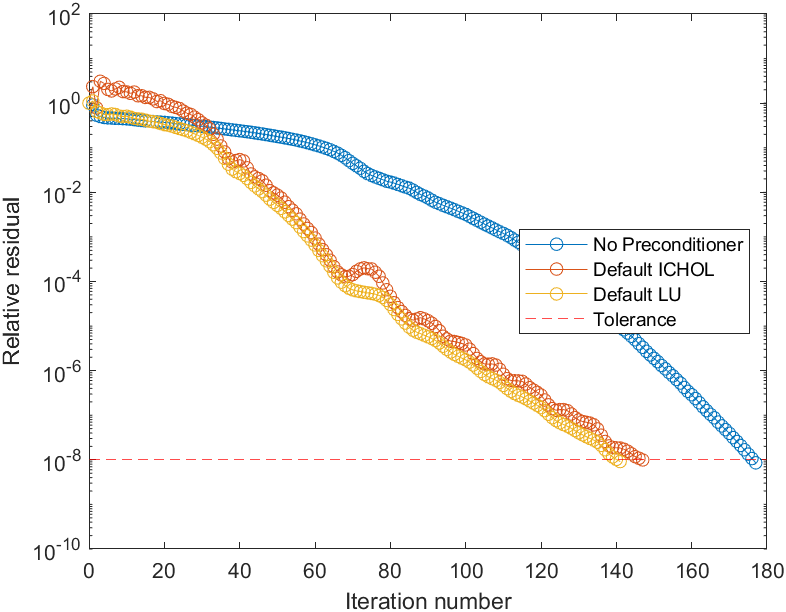
\includegraphics[scale=0.70]{img/dupcova/qmr}}
    \caption{История невязок методом qmr для матрицы Dubcova2}
    \label{fig:image_9}
\end{figure}

\begin{figure}[H]
    \renewcommand{\figurename}{Рисунок}
    \centering{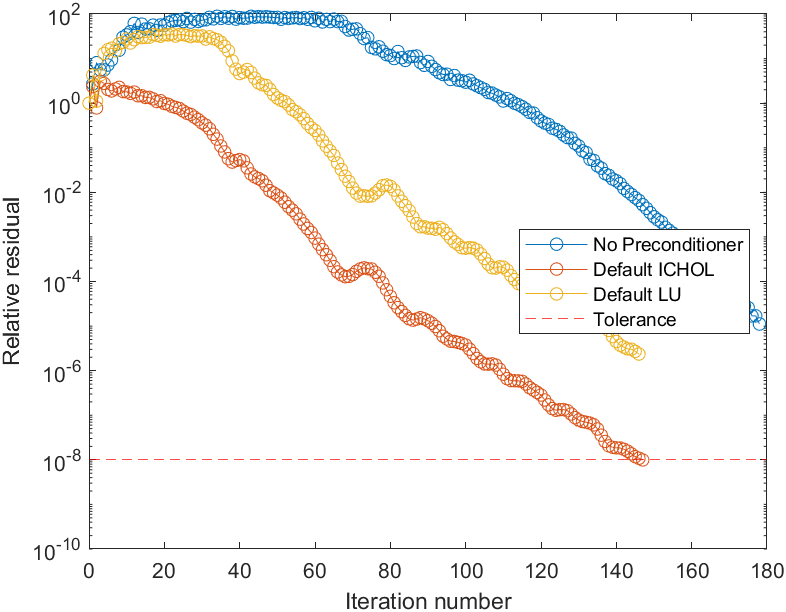
\includegraphics[scale=0.70]{img/dupcova/symmlq}}
    \caption{История невязок методом symmlq для матрицы Dubcova2}
    \label{fig:image_10}
\end{figure}

\begin{figure}[H]
    \renewcommand{\figurename}{Рисунок}
    \centering{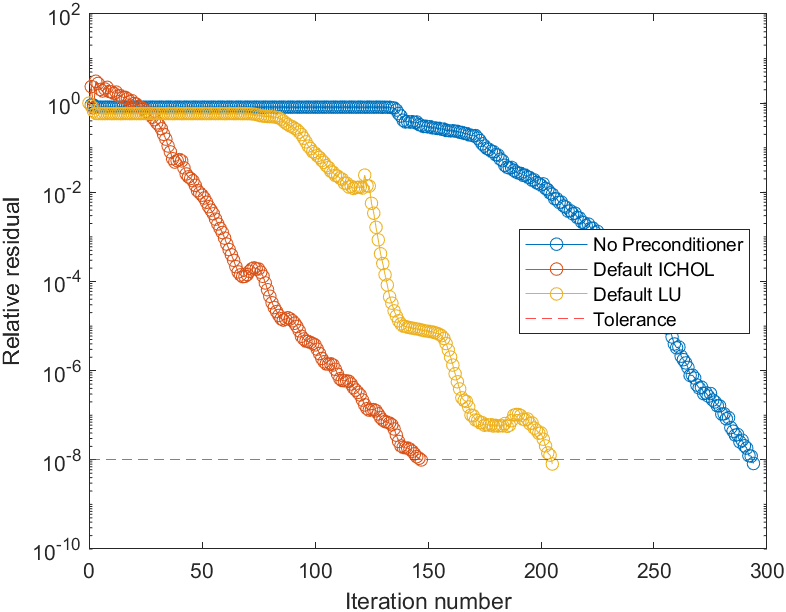
\includegraphics[scale=0.70]{img/dupcova/tfqmr}}
    \caption{История невязок методом tfqmr для матрицы Dubcova2}
    \label{fig:image_11}
\end{figure}


В таблице 2 приведена сводная информация о использовании каждого метода для матрицы Dubcova2

\begin{table}[H]
    \renewcommand{\tablename}{Таблица}
    \caption{сравнение методов по точности и количеству итерацй для матрицы Dubcova2}
    \label{tab:table1}
    \begin{tabularx}{1\textwidth}{
        | >{\centering\arraybackslash}X
        | >{\centering\arraybackslash}X
        | >{\centering\arraybackslash}X
        | >{\centering\arraybackslash}X
        | >{\centering\arraybackslash}X
        | >{\centering\arraybackslash}X
        | >{\centering\arraybackslash}X |
    }
        \hline
        \multirow{Название метода} &
        \multicolumn{2}{X|}{Без предобуславливателя} &
        \multicolumn{2}{X|}{С предобуславливателем неполное разложение Холецкого} &
        \multicolumn{2}{X|}{С предобуславливателем LU-разложение} \\
        \cline{2-7}
        & Число итераций & Точность & Число итераций & Точность & Число итераций & Точность \\
        \hline
        bicg & 180 & $10^{-8}$ & 148 & $10^{-8}$ & 148 & $10^{-8}$  \\
        \hline
        bicgstab & 250 & $10^{-8}$ & 148 & $10^{-8}$ & 204 & $10^{-8}$ \\
        \hline
        bicgstabl & 270 & $10^{-8}$ & 150 & $10^{-8}$ & 180 & $10^{-8}$ \\
        \hline
        cgs & 152 & $10^{-8}$ & 148 & $10^{-8}$ & 104 & $10^{-8}$ \\
        \hline
        gmres & 180 & $10^{-8}$ & 148 & $10^{-8}$ & 147 & $10^{-8}$ \\
        \hline
        lsqr & 2000 & $10^{-8}$ & 144 & $10^{-8}$ & 2300 & $10^{-8}$ \\
        \hline
        minres & 180 & $10^{-8}$ & 147 & $10^{-8}$ & 140 & $10^{-8}$ \\
        \hline
        pcg & 180 & $10^{-8}$ & 147 & $10^{-8}$ & 147 & $10^{-8}$ \\
        \hline
        qmr & 178 & $10^{-8}$ & 145 & $10^{-8}$ & 147 & $10^{-8}$ \\
        \hline
        symmlq & 180 & $10^{-5}$ & 149 & $10^{-6}$ & 148 & $10^{-6}$ \\
        \hline
        tfqmr & 290 & $10^{-8}$ & 150 & $10^{-8}$ & 216 & $10^{-8}$ \\
        \hline
    \end{tabularx}
\end{table}



Из таблицы 2 видно, что минимальное количество итераций при приемлемой точности получилось
у всех методов с предобуславливателем неполное разложение Холецкого (от 145 до 150 итераций).
Самое большое количество итераций понадобилось методу lsqr с предобуславливателем LU-разложение (2300 итераций).
Матрица не смогла посчитаться методом symmlq с установленной точностью (10^{-6}  вместо 10^{-8}).

На рисунках 12--22 приведены истории невязок для матрицы Qa8fm

\begin{figure}[H]
    \renewcommand{\figurename}{Рисунок}
    \centering{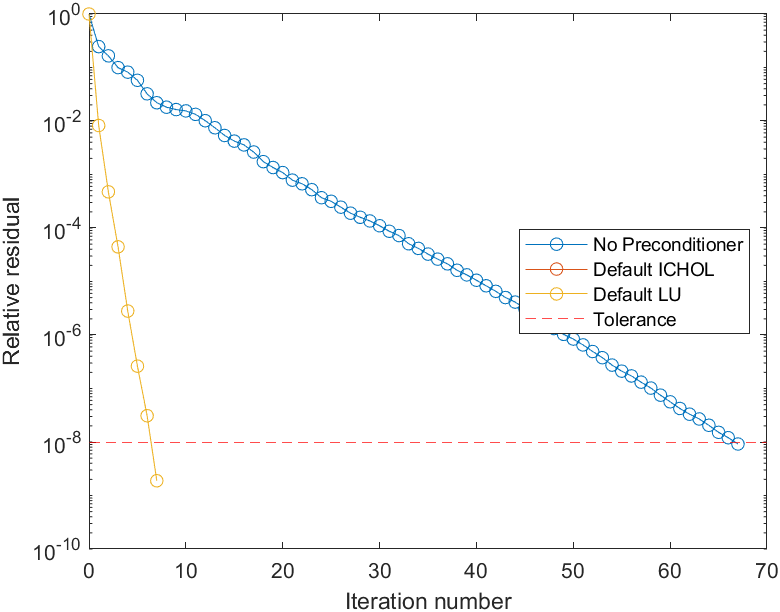
\includegraphics[scale=0.70, inner]{img/qa8fm/bicg}}
    \caption{История невязок методом bicg для матрицы Qa8fm}
    \label{fig:image_12}
\end{figure}

\begin{figure}[H]
    \renewcommand{\figurename}{Рисунок}
    \centering{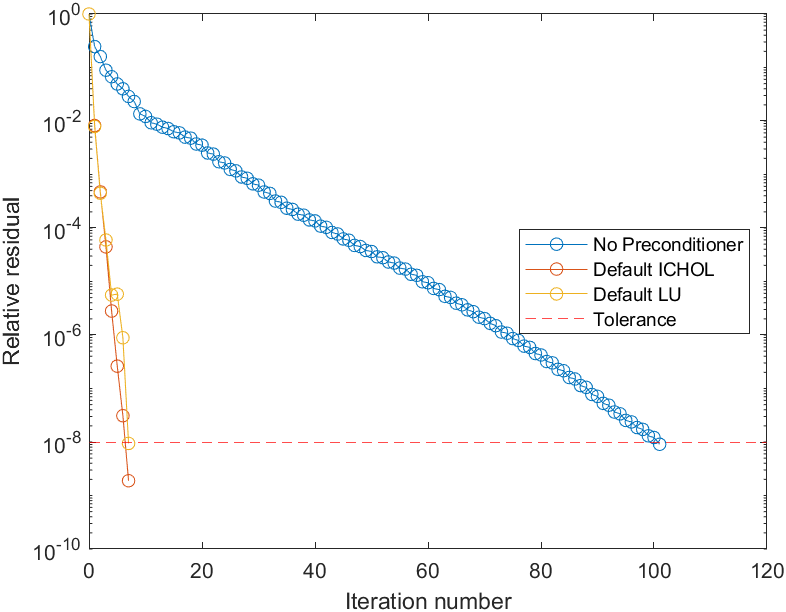
\includegraphics[scale=0.70]{img/qa8fm/bicgstab}}
    \caption{История невязок методом bicgstab для матрицы Qa8fm}
    \label{fig:image_13}
\end{figure}

\begin{figure}[H]
    \renewcommand{\figurename}{Рисунок}
    \centering{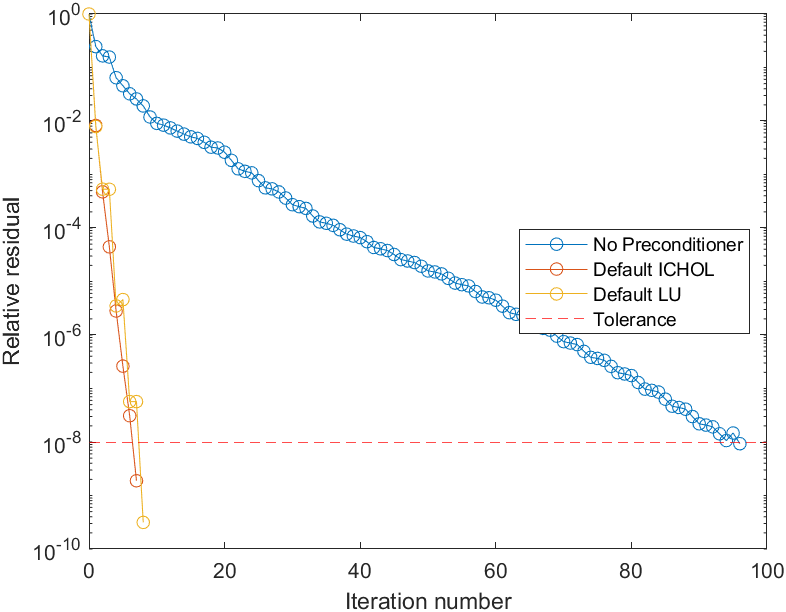
\includegraphics[scale=0.70]{img/qa8fm/bicgstabl}}
    \caption{История невязок методом bicgstabl для матрицы Qa8fm}
    \label{fig:image_14}
\end{figure}

\begin{figure}[H]
    \renewcommand{\figurename}{Рисунок}
    \centering{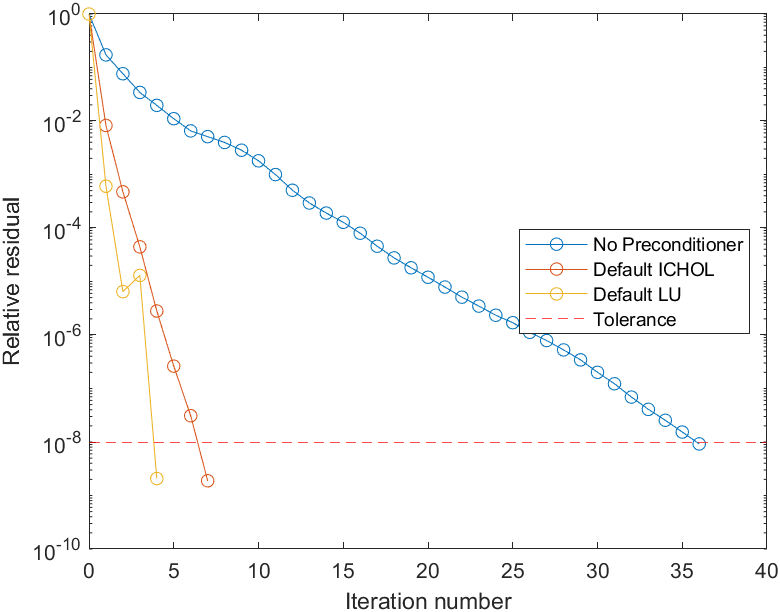
\includegraphics[scale=0.70]{img/qa8fm/cgs}}
    \caption{История невязок методом cgs для матрицы Qa8fm}
    \label{fig:image_15}
\end{figure}

\begin{figure}[H]
    \renewcommand{\figurename}{Рисунок}
    \centering{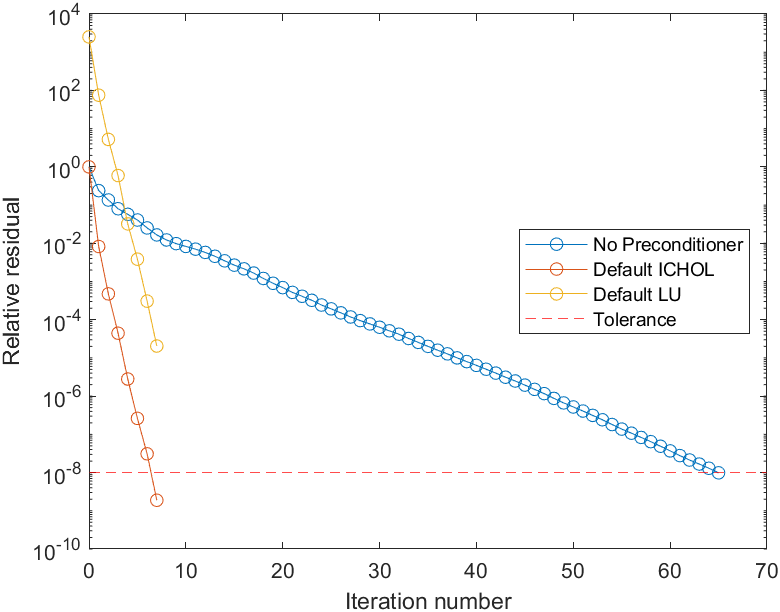
\includegraphics[scale=0.70]{img/qa8fm/gmres}}
    \caption{История невязок методом gmres для матрицы Qa8fm}
    \label{fig:image_16}
\end{figure}

\begin{figure}[H]
    \renewcommand{\figurename}{Рисунок}
    \centering{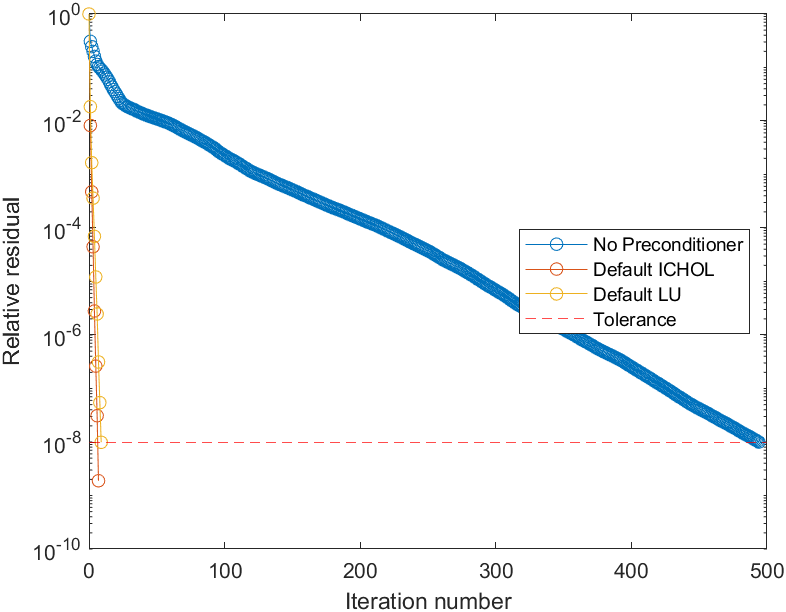
\includegraphics[scale=0.70]{img/qa8fm/lsqr}}
    \caption{История невязок методом lsqr для матрицы Qa8fm}
    \label{fig:image_17}
\end{figure}

\begin{figure}[H]
    \renewcommand{\figurename}{Рисунок}
    \centering{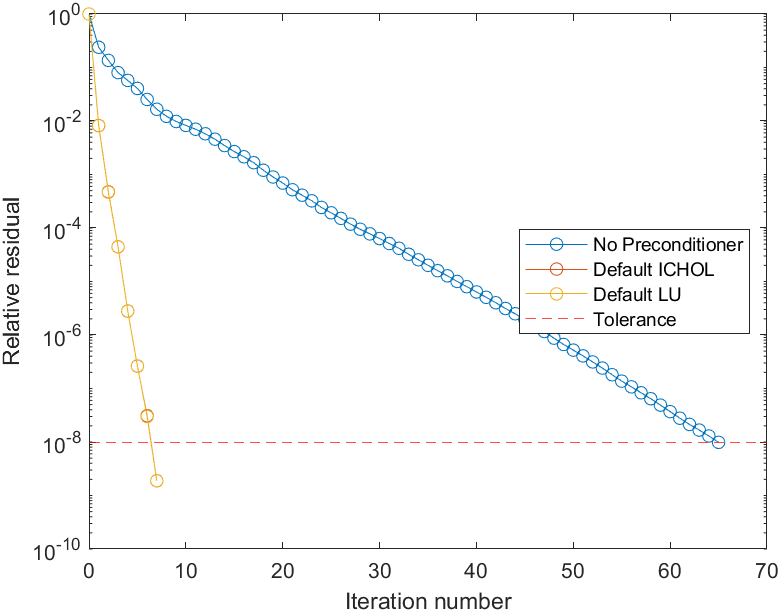
\includegraphics[scale=0.70]{img/qa8fm/minres}}
    \caption{История невязок методом minres для матрицы Qa8fm}
    \label{fig:image_18}
\end{figure}

\begin{figure}[H]
    \renewcommand{\figurename}{Рисунок}
    \centering{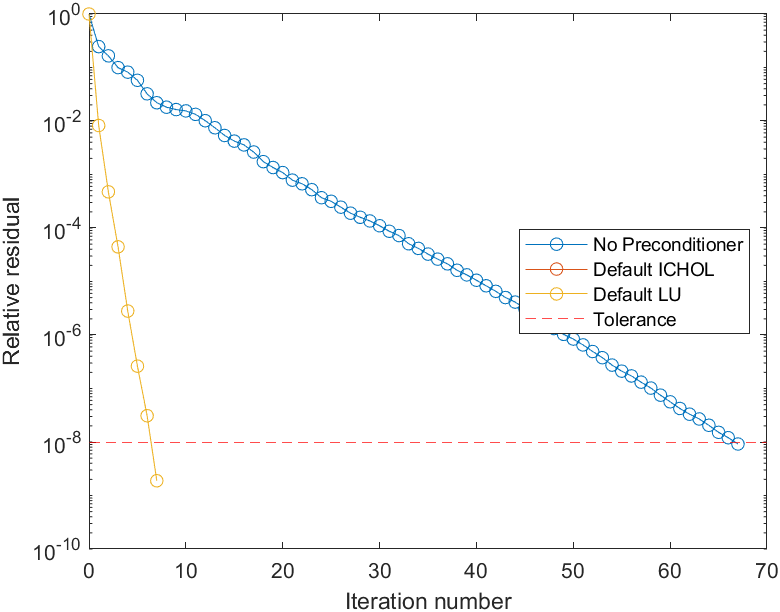
\includegraphics[scale=0.70]{img/qa8fm/pcg}}
    \caption{История невязок методом pcg для матрицы Qa8fm}
    \label{fig:image_19}
\end{figure}

\begin{figure}[H]
    \renewcommand{\figurename}{Рисунок}
    \centering{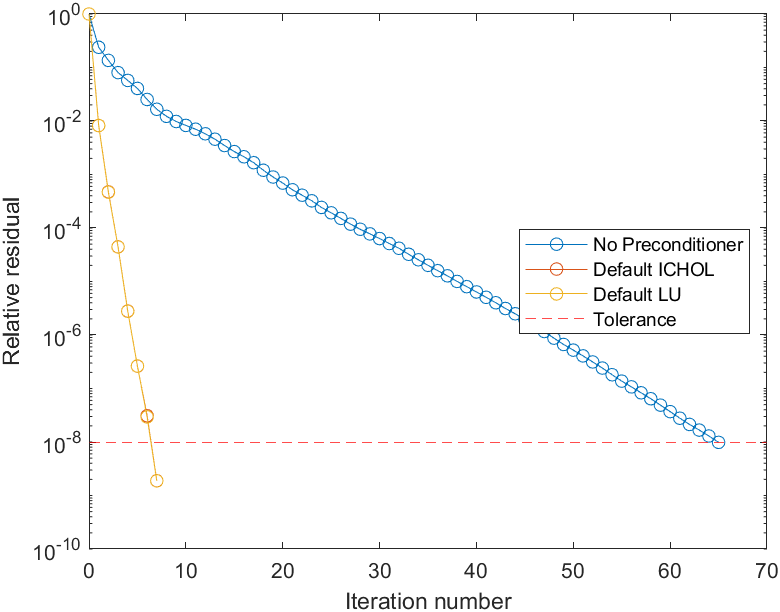
\includegraphics[scale=0.70]{img/qa8fm/qmr}}
    \caption{История невязок методом qmr для матрицы Qa8fm}
    \label{fig:image_20}
\end{figure}

\begin{figure}[H]
    \renewcommand{\figurename}{Рисунок}
    \centering{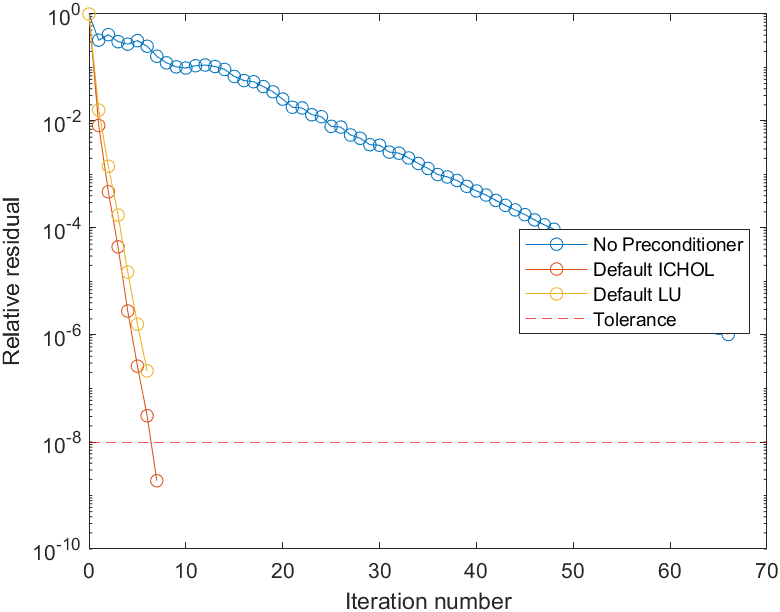
\includegraphics[scale=0.70]{img/qa8fm/symmlq}}
    \caption{История невязок методом symmlq для матрицы Qa8fm}
    \label{fig:image_21}
\end{figure}

\begin{figure}[H]
    \renewcommand{\figurename}{Рисунок}
    \centering{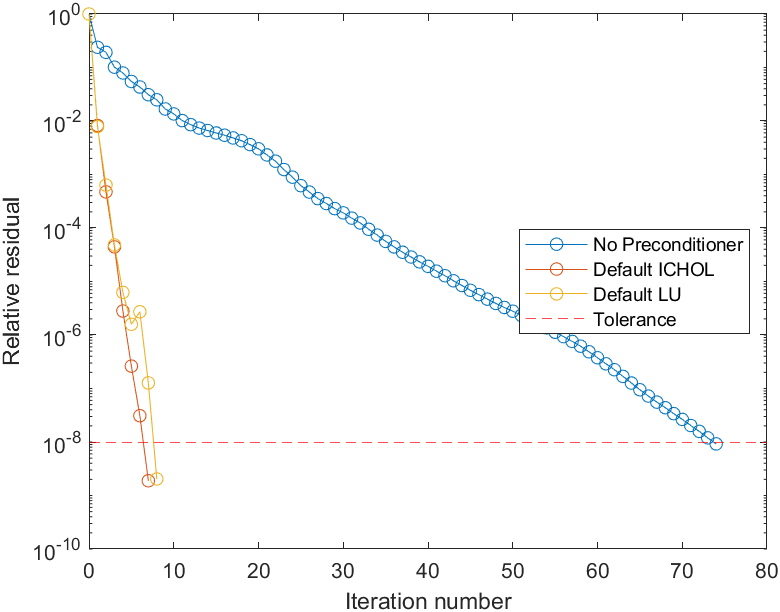
\includegraphics[scale=0.70]{img/qa8fm/tfqmr}}
    \caption{История невязок методом tfqmr для матрицы Qa8fm}
    \label{fig:image_22}
\end{figure}


В таблице 3 приведена сводная информация о использования каждого метода для матрицы Qa8fm.

\begin{table}[H]
    \renewcommand{\tablename}{Таблица}
    \caption{cравнение методов по точности и количеству итераций для матрицы Qa8fm}
    \label{tab:table3}
    \begin{tabularx}{1\textwidth}{
        | >{\centering\arraybackslash}X
        | >{\centering\arraybackslash}X
        | >{\centering\arraybackslash}X
        | >{\centering\arraybackslash}X
        | >{\centering\arraybackslash}X
        | >{\centering\arraybackslash}X
        | >{\centering\arraybackslash}X |
    }
        \hline
        \multirow{Название метода} &
        \multicolumn{2}{X|}{Без предобуславливателя} &
        \multicolumn{2}{X|}{С предобуславливателем неполное разложение Холецкого} &
        \multicolumn{2}{X|}{С предобуславливателем LU-разложение} \\
        \cline{2-7}
        & Число итераций & Точность & Число итераций & Точность & Число итераций & Точность \\
        \hline
        bicg        &  68 & $10^{-8}$ & 8 & $10^{-8}$ & 8 & $10^{-8}$  \\
        \hline
        bicgstab    & 100 & $10^{-8}$ & 8 & $10^{-8}$ & 9 & $10^{-8}$ \\
        \hline
        bicgstabl   & 95 & $10^{-8}$ & 8 & $10^{-8}$ & 9 & $10^{-8}$ \\
        \hline
        cgs         & 36 & $10^{-8}$ & 8 & $10^{-8}$ & 4 & $10^{-8}$ \\
        \hline
        gmres       & 65 & $10^{-8}$ & 8 & $10^{-8}$ & 10 & $10^{-5}$ \\
        \hline
        lsqr        & 500 & $10^{-8}$ & 8 & $10^{-8}$ & 9 & $10^{-8}$ \\
        \hline
        minres      & 65 & $10^{-8}$ & 8 & $10^{-8}$ & 8 & $10^{-8}$ \\
        \hline
        pcg         & 67 & $10^{-8}$ & 8 & $10^{-8}$ & 8 & $10^{-8}$ \\
        \hline
        qmr         & 64 & $10^{-8}$ & 8 & $10^{-8}$ & 8 & $10^{-8}$ \\
        \hline
        symmlq      & 67 & $10^{-6}$ & 7 & $10^{-8}$ & 8 &$ 10^{-7}$ \\
        \hline
        tfqmr       & 75 & $10^{-8}$ & 7 & $10^{-8}$ & 8 & $10^{-8}$ \\
        \hline
    \end{tabularx}
\end{table}


Из таблицы 3 видно, что в среднем всем методам спредобуславливателем понадобилось примерно одинаковое количество
итераций (в среднем 8).
Самое большое количество итераций понадобилось методу lsqr без предобуславливателя (500 итераций).

На рисунках 23-32 приведены истории невязок для матрицы Thermomech_dM

